\chapter{HIGGS BOSON MASS MEASUREMENT IN THE \texorpdfstring{\hzzfourl}{H to ZZ to 4l} CHANNEL}
\label{ch:higgs_mass}
% Need to use \texorpdfstring{} so it also shows in pdf bookmarks.
\section{Motivation}
\label{sec:higgs_motivation}
When the CMS and ATLAS collaborations announced the discovery of the Higgs boson on July 4, 2012,
% TODO: Add higgs production modes here?
% TODO: Include ref to HIG-21-019 somewhere around here?
this was a momentous achievement in particle physics because the so-called ``missing'' piece of the SM was found~\cite{chatrchyan_observation_2012, ATLAS:2012yve, chatrchyan_observation_2013}.
Evidence of the Higgs boson's existence also motivates the associated Higgs field, which permeates all of spacetime and explains the origins of the masses of all the other massive fundamental particles (Chapter~\ref{ch:theory}).

The Higgs boson is interesting for a variety of reasons.
First, it is currently one of a kind---the only fundamental scalar particle ever discovered at the time of this writing.
Second, the mass of the Higgs boson theoretically determines the stability of our very Universe (Fig.~\ref{fig:universe_stability}).
Third, the unique boson could be a portal to new physics---\ie physics beyond the Standard Model (BSM)---\eg by decaying into BSM low-mass dilepton mass resonances (Chapter~\ref{ch:dilep_res}).
Fourth, the Higgs boson may not be the only one of its kind; some BSM models theorize that other kinds of Higgs bosons may exist~cite{Branco:2011iw}.
Fifth, \emph{are we certain that the Higgs boson discovered in 2012 is the same as the one predicted by the SM?}
To check this, it is necessary to compare the Higgs boson's measured properties to its predicted ones.
One such property is the mass of the Higgs boson $\left( \mH \right)$.

Although many previous measurements of \mH have already been made (\eg by the ATLAS and CMS collaborations as shown in \cref{fig:atlas_cms_mH_meas}), this chapter presents a recipe for the measurement of \mH that is predicted to give the world's most precise value of \mH to date, once the data are unblinded.
%=== ATLAS and CMS measurements of mH.
%%%%%%%%%%%%%%%%%%%%
\begin{multiFigure}
    \centering
        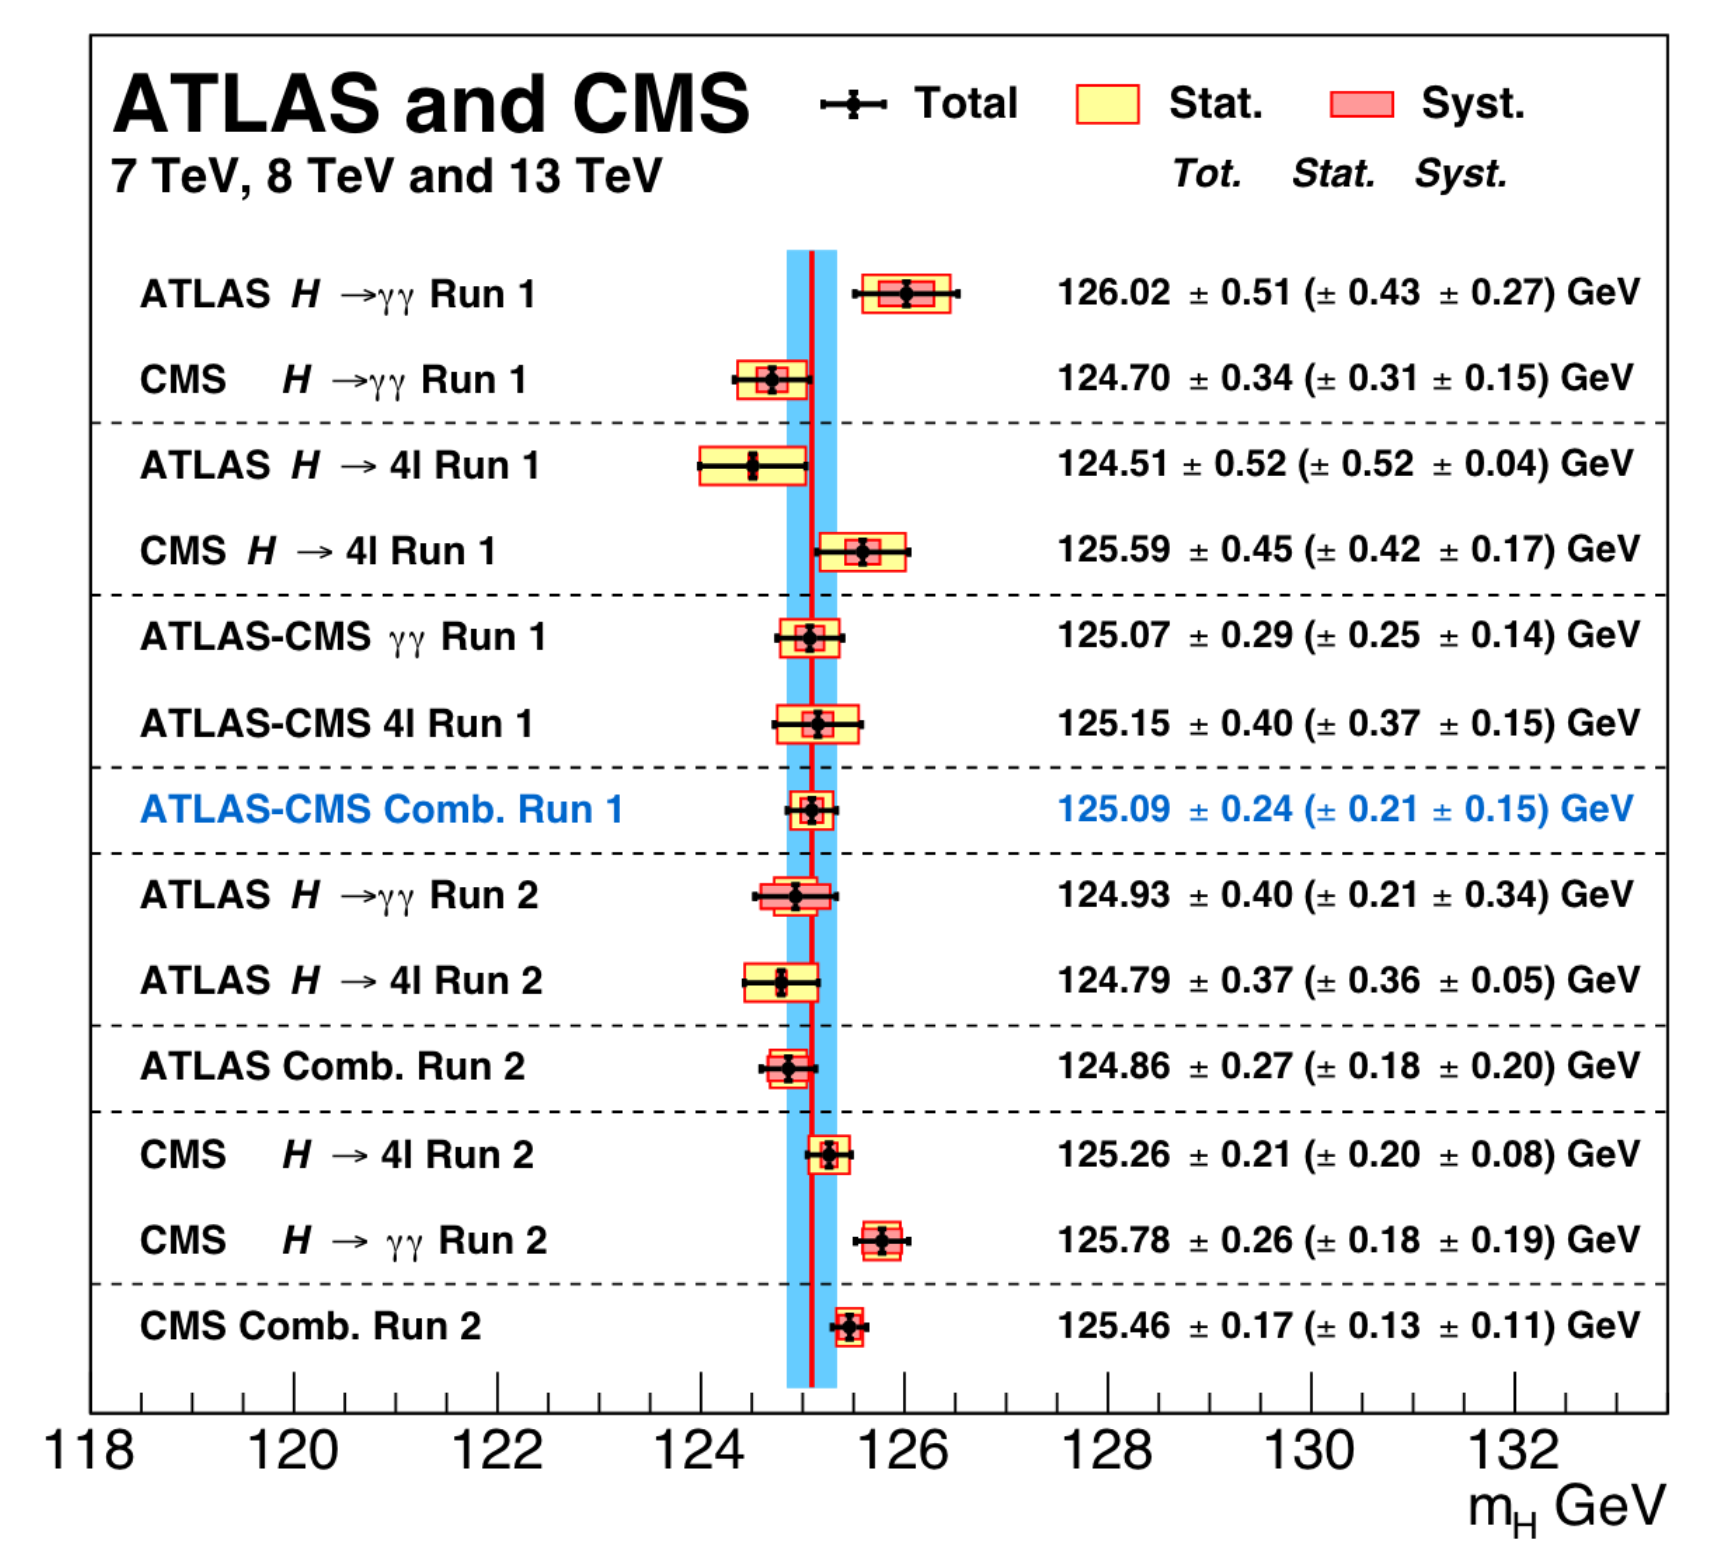
\includegraphics[width=\textwidth,keepaspectratio]{figures/higgsmassmeas/all_mH_measurements_atlas_cms.png}
    \captionof{figure}
        [Various measurements of \mH made by the CMS and ATLAS collaborations]
        {Various measurements of \mH made by the CMS and ATLAS collaborations in the \htoyy and \hzzfourl channels, during Runs 1 and 2 of the LHC.
        Plot taken from~\cite{particle_data_group_review_2020}.}
    \label{fig:atlas_cms_mH_meas}
\end{multiFigure}
%%%%%%%%%%%%%%%%%%%%
% Some properties of the Higgs boson can be predicted by the SM, like 
%     - There are many results on Higgs properties: spin, charge, decay processes, lifetime, mass.
%     - The last of these is the focus of this dissertation and is of particular importance to the Universe: depending on mH and mtop, the stability of the Universe.
% - Why this thesis is important:
%     - This thesis describes the methodology and results of the best precision measurement of mH to date by using the hZZ4l decay and Full Run 2 data set from CMS.
%     - Run 2 provides more data -> more precision on measurements of Higgs properties.
%     - In addition to more HZZ4l events, this analysis provides new techniques, specifically the VX constraint.
%     - Predict mH for Run 3, will start soon summer 2022 and provide an approximate 300? /fb of L int.
%     - In 2026(?), HLLHC provides even more data. ref snowmass paper.
The estimate for the lowest uncertainties on \mH comes from the following improvements compared to previous measurements:
\begin{itemize}
    % More data.
    \item Nearly four times as much collected data from Run 2 $\left( \lumiint = \lumiruntwo \right)$ \vs the data used for the 2016 measurement $\left( \lumiint = \lumisixteen \right)$.
    % Four final states (instead of three).
    \item Four final-state categories: \fourmu, \foure, \twoetwomu, \twomutwoe.
    In previous measurements, the last two final states (the mixed-flavor states) were combined, when truly they have different kinematical properties (depending on into which lepton pair the \Zone decayed):
    different peak widths (instrumental resolutions), different signal efficiencies, and different relative levels of reducible background.
    % Using UL reco (better electron pT resolution).
    \item Ultra-Legacy (UL) reconstruction for muon, electron, photon, and jet tracks.
    This signficantly improves electron momenta and improves the other particle momenta, though to a lesser degree.
    % Vertex constraint.
    \item The measurements of muon \pt are improved by constraining the muon tracks to originate from the interaction vertex (also called a \emph{vertex+beamspot constraint}).
    \item When extracting the value of \mH in past measurements, a 3D $\text{pdf} \left( \mfourl, \mfourlerr, \Dkinbkg \right)$ was built into a factorized form
    $f \left( \mfourl, \mfourlerr \middlepipe \mH \right)   \cdot   g\left( \Dkinbkg \middlepipe \mfourl \right)$,
    which was later found to contain an existing correlation between \mfourlerr and \Dkinbkg.
    To account for this correlation, now the events are split into 9 categories based on the per-event \emph{relative} mass uncertainty $\left( \relmfourlerr \right)$ and, for each, a 2D $\text{pdf} \left( \mfourl, \Dkinbkg \middlepipe \mh \right)$ is built.
    % Z1 mass constraint.
    % The improvement here is that now the muon tracks are constrained to come from the interaction vertex in the fit (sometimes called a \emph{vertex constraint}).
    \item The systematic uncertainties on electron and muon momentum scales $\left( \pt^{\Pe, \Pmu} \right)$ are reduced, thanks to a more detailed analysis on the uncertainties.
    This has the additional effect of significantly reducing the uncertainty on the per-event four-lepton mass resolution.
\end{itemize}

The layout of the remainder of this chapter is as follows:
First, a general overview of the logic and analysis workflow for the \mH measurement is motivated in \cref{sec:analysis_overview}.
The specific data sets, simulated samples, and triggers used in the analysis are then detailed in \cref{sec:analyzed_data}.
Then the event reconstruction and event selection are described in \cref{sec:evt_sel}.
Afterwards, an analysis of the background estimation is given in \cref{sec:bkg_estim}.
The signal modeling and improvements utilized in this measurement are then laid out, which include the kinematic discriminant, per-event mass uncertainties, and the vertex constraint in \cref{sec:signal_model}.
A treatment of the systematic uncertainties follows in \cref{sec:syst_uncert}.
The chapter concludes with the expected uncertainties on the \mH measurement in \cref{sec:results}, considering Full Run 2 data from the LHC.

% \begin{itemize}                                                                          
%     \item Sec.~\ref{sec:analysis_overview}: General overview of the analysis of the Higgs boson mass measurement.
%     \item Sec.~\ref{sec:analyzed_data}: Data sets, triggers, and simulation.
%     \item Sec.~\ref{sec:evt_sel}: Event reconstruction and selection.
%     \item Sec.~\ref{sec:bkg_estim}: Background estimation.
%     \item Sec.~\ref{sec:signal_model}: Signal modeling and improvements, including kinematic discriminant, per-event mass uncertainties, VXBS constraint, reference to ad hoc studies in appendix.
%     % \item Observables: Four-Lepton Invariant Mass, Per-Event Mass Uncertainty, Matrix Element-Based Kinematic Discriminant) (Sec.~\ref{sec:observables})
%     \item Sec.~\ref{sec:syst_uncert}: Systematic uncertainties.
%     \item Sec.~\ref{sec:results}: Results.
% \end{itemize}
